\documentclass[11pt]{article}

\usepackage{ppackage}
\usepackage{bbm}
\usepackage{import}






\usepackage{tikz}
\usetikzlibrary{arrows.meta,patterns}
\usetikzlibrary{ipe} % ipe compatibility library

\usepackage{../../Notes/tikzit}
\usepackage{../../Notes/utf8math}
\usetikzlibrary{positioning, 
                quotes}

\input{../../Notes/TIKZ/digraph.tikzstyles}



\usepackage{url}


\newcommand{\solution}{
\bigskip\noindent
	\textbf{Solution: \\}}
	


\DeclareMathOperator{\size}{size}
\DeclareMathOperator{\conv}{conv}
\newcommand{\SV}{\mathrm{SV}}
\newcommand{\bigO}{O}
\newcommand{\cut}{\mathrm{cut}}
\newcommand{\LLL}{\mathrm{LLL}}
\newcommand{\setR}{\mathbb{R}}
\newcommand{\setZ}{\mathbb{Z}}
\newcommand{\setQ}{\mathbb{Q}}
\newcommand{\setC}{\mathbb{C}}
\newcommand{\setN}{\mathbb{N}}
\newcommand{\wt}[1]{\widetilde{#1}}
\newcommand{\opt}{{\sc 0/1-opt}\xspace}
\newcommand{\aug}{{\sc 0/1-aug}\xspace}
\newcommand{\psep}{{\sc 0/1-psep}\xspace}
\newcommand{\sep}{{\sc 0/1-sep}\xspace}
\newcommand{\fopt}{{\sc 0/1-testopt\xspace} }

\newcommand{\hpp}{\mathrm{HPP}}
\newcommand{\nodes}{\mathcal{V}}
\newcommand{\vol}{\mathrm{vol}}
\newcommand{\diag}{\mathrm{diag}}
\newcommand{\arcs}{\mathcal{A}}
\newcommand{\edges}{\mathcal{E}}
\newcommand{\paths}{\mathscr{P}}
\newcommand{\cycles}{\mathcal{C}}




\newcommand{\K}{{\mathcal K}}
\newcommand{\A}{{A}}
\newcommand{\B}{{B}}
\newcommand{\T}{\mathscr{T}}
\newcommand{\eE}{\mathscr{E}}
\newcommand{\eS}{\mathscr{S}}
\newcommand{\eP}{\mathscr{P}}
\newcommand{\eM}{\mathscr{M}}



\newcommand{\transp}{^{\mathrm{T}}}

\newcommand{\smallmat}[1]{\left( \begin{smallmatrix} #1 \end{smallmatrix}\right)}

\newcommand{\mat}[1]{ \begin{pmatrix} #1 \end{pmatrix}}
\newcommand{\smat}[1]{ \big(\begin{smallmatrix} #1 \end{smallmatrix}\big)}

\newcommand{\pc}{\mathscr{P}}
\newcommand{\ob}{\mathscr{O}}
\newcommand{\odds}{\mathscr{W}}
\newcommand{\up}{\mathscr{U}}
\newcommand{\ef}{\mathscr{F}}
\newcommand{\eh}{\mathscr{H}}
\newcommand{\ev}{\mathscr{V}}
\newcommand{\ec}{\mathscr{C}}
\newcommand{\eu}{\mathscr{U}}

\newcommand{\lex}{\mathrm{lex}}

\renewcommand{\leq}{\leqslant}
\renewcommand{\geq}{\geqslant}









\newcommand{\linhull}{\mathrm{lin.hull}}
\newcommand{\affhull}{\mathrm{affine.hull}}
\newcommand{\charcone}{\mathrm{char.cone}}
\newcommand{\cone}{\mathrm{cone}}
\newcommand{\rank}{\mathrm{rank}}
\newcommand{\wb}[1]{\overline{#1}}



\usepackage{enumerate}

      
\institute{\'Ecole Polytechnique F\'ed\'erale de Lausanne}
\lecture{Discrete Optimization}
\faculty{Prof. Eisenbrand}
\term{Spring 2025}
\publishdate{May 6, 2025}
\duedate{ }
\problemset{Assignment~11}

\begin{document}
\makeheader

\begin{enumerate}[1)]
\item Find a maximum cardinality matching and a minimum cardinality vertex cover in the following graph.
  \begin{center}
    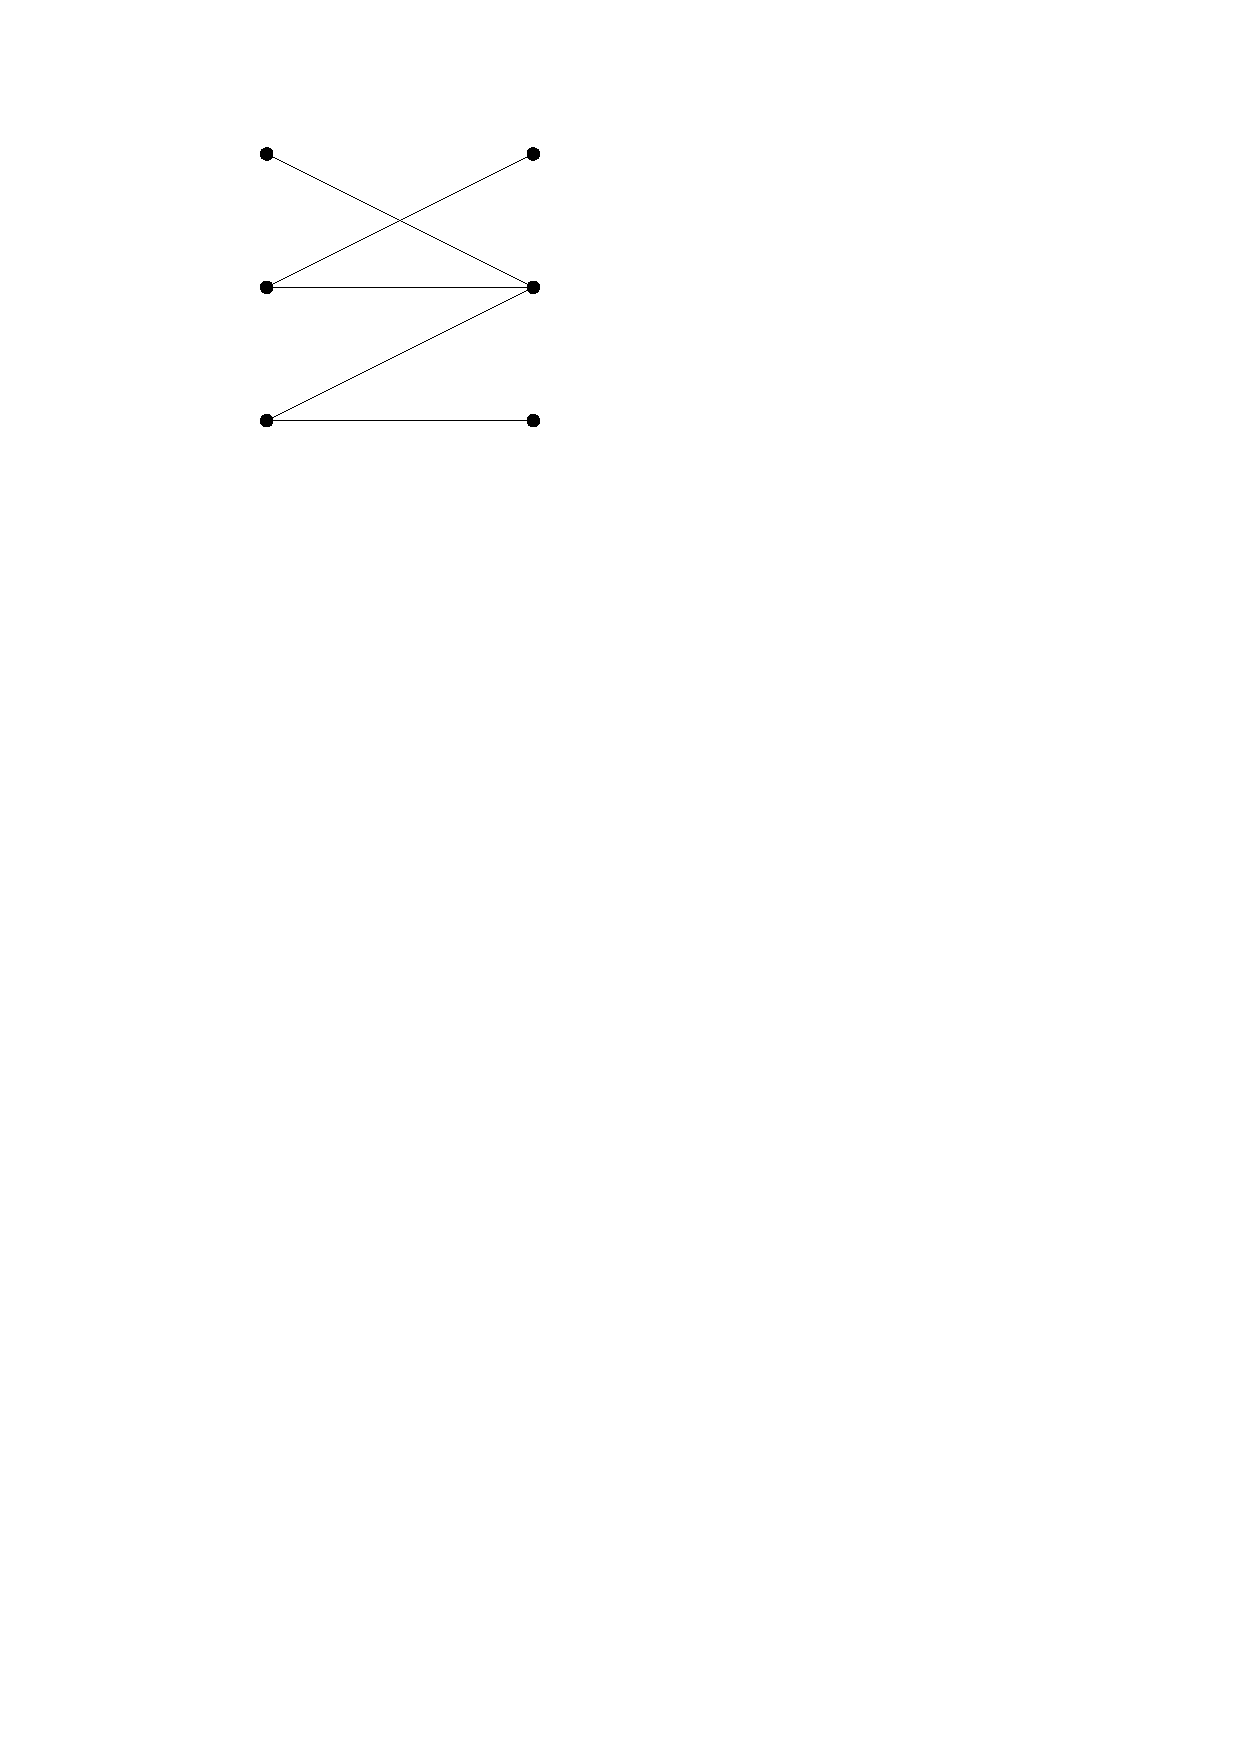
\includegraphics[width=0.2\textwidth]{graph1}
  \end{center}
\item 
Let $A \in \R^{n \times n}$ be an invertible matrix and $b \in \R^{n}$ a vector. The ellipsoid $E(A,b)$ is defined as the image of the unit ball under the linear mapping $t(x) = Ax+b$. Show that
$$E(A,b) = \{ x \in \R^n: (x-b)^\top A^{-\top} A^{-1} (x-b) \leq 1 \}.$$
	
\item 
Draw $E(A,b)$ for $A = \begin{pmatrix} 1 & 3  \\ 2 & 5 \end{pmatrix}$ and $b  = \begin{pmatrix} 1   \\ 2 \end{pmatrix}$. What are the axes of $E(A,b)$?

\item Let $D = (V,A)$  be a directed graph and $A_D ∈ \{0,\pm1\}^{|V| × |A|}$ be the node-edge incidence matrix of $D$. Assume that the underlying undirected graph $G = (V,E)$  with $E = \{ uv : uv ∈A \text{ or } vu ∈ A\}$ is connected. 
  \begin{enumerate}[i)]
  \item Show that any row of $A_D$ is in the span of the other rows.
  \item Let $T ⊆ A$ be a selection of $n-1$ arcs of $A$ such that the induced undirected graph is a spanning tree of $G$. Show that the corresponding columns of $A_D$ are linearly independent.
  \end{enumerate}
  
  
  
\item Let $f \in \mathbb{R}^{|A|}_{\geq 0}$ be a flow of a directed graph. Show that we can find a feasible flow $f^*$ such that $f^* = \sum_{p \in P}  \mu_p \cdot p + \sum_{c \in C}\mu_c \cdot c$ where $C$ is a set of cycles in the graph, $P$ is a set of paths in the graph, and $\mu_l, \mu_p \in \mathbb{R}_{\geq 0}$.

\medskip 

\paragraph{Example:}

\begin{figure}[h!]
    \centering
    \begin{tikzpicture}[node distance=2cm,
    B/.style={circle, draw, minimum size=.8cm},
    edge/.style={->,> = latex', font=\footnotesize}]
    
    \node[B] (s) at (0, 0) {$s$};
    \node[B](a) at (2, 1){$a$};
    \node[B](c) at (2, -1){$c$};
    \node[B](b) at (4, 1){$b$};
    \node[B](d) at (4, -1){$d$};
    \node[B](t) at (6, 0){$t$};
   \node (a2) at (2.1, 1){};
   \node (c2) at (2.1, -1){};
   \node (b2) at (4.1, 1){};
   \node (d2) at (4.1, -1){};
    
    \draw[edge] (s) to node[midway ] {$7/10$} (a);
    \draw[edge] (s) to node[midway ] {$8/10$} (c);
    \draw[edge] (a2) to node[above left] {$0/4$} (c2);
    \draw[edge] (c) to node[below right] {$2/5$} (a);
    \draw[edge] (a) to node[midway ] {$5/5$} (b);
    \draw[edge] (b) to node[midway ] {$0/7$} (c);
    \draw[edge] (b2) to node[above left ] {$0/10$} (d2);
    \draw[edge] (c) to node[midway ] {$10/10$} (d);
    \draw[edge] (d) to node[below right ] {$2/6$} (b);
    \draw[edge] (b) to node[midway ] {$3/3$} (t);
    \draw[edge] (d) to node[midway ] {$12/14$} (t);
    




    
    %\draw (s) -- (a) node[midway, fill=white]{$7/10$};
    %\draw (s) -- (c){$8/10$};
    %\draw (a) -- (c){$0/4$};
    %\draw (c) -- (a){$2/5$};    
    
    
    
    \end{tikzpicture}
    \end{figure}
    
    
    

This flow can be decomposed into the following combination of paths:\\
•$p1: s →a →b →t$ ($f1$ assigns $3$ units to each edge in $p1$)\\
•$p2: s →c →d →t$ ($f2$ assigns $8$ units to each edge in $p2$)\\
•$p3: s →a →b →d →t$ ($f3$ assigns $2$ units to each edge in $p3$)\\
•$p4: s →a →c →d →t$ ($f4$ assigns $2$ units to each edge in $p4$)



\item Let $D= (V,A)$ be a digraph. For every $a∈A$, let $l_a, u_a \in \mathbb{R}_{\geq 0}$ be given such that $l_a \leq u_a$. Show that
the set of circulations $\{x∈\setR^A : A_Dx= 0, l \leq x \leq u \}$ (with $A_D$ being the node-arc incidence matrix of $D$) is nonempty if and only if
$$ \displaystyle\sum_{a \in \delta^-(X)} l_a \leq \displaystyle\sum_{a \in \delta^+(X)} u_a \quad \text{for all }X \subseteq V. $$



\end{enumerate}




  

\end{document}

%%% Local Variables:
%%% mode: latex
%%% TeX-master: t
%%% End:
